\chapter{Results}\label{chap:results}

We have plugged this method into the~real-time planet renderer which we already mentioned in the~introduction. With this method, we compressed and then real-time viewed the~whole-Earth height data with 90m span between height samples (SRTM). The~total size of this dataset is 58~GB. Due to the~data redundancy of the~LOD hierarchy of the~renderer which is caused by the~fact that it stores all LODs of terrain completely separately, the~total size of the~SRTM dataset converted to this hierarchy was 260GB. When we applied this compression method to every independent square node of this LOD hierarchy, we managed to compress this data down to 7GB with the~maximum deviation of the~compression set to 5m. This yield the~compression ratio of 37:1. However, if we take the~size of the~original SRTM dataset as the~original size, the~compression ratio will drop to just about 8:1. It needs to be said that the~first ratio is solely the~credit of our method, whereas the~second one is influenced by both the~way the~renderer handles the~data and our method. 

For a~comparison, C-BDAM achieved the~compression ratio of 64:1 on the~same 90m-resolution SRTM dataset with the~maximum error bound set to 16m. As we already mentioned, C-BDAM contains its own LOD rendering hierarchy without any redundancy - a~finer LOD is constructed from the~coarser one which is where the~compression takes place. Thanks to this, there is no data redunduncy in the~LOD hierarchy of C-BDAM, so the~compression ratio of this method was evaluated with respect to the~original size of the~dataset which is 58~GB. The~final size of the~compressed data prepared for rendering in C-BDAM was just 870MB.

The~most accurate comparison of our method with C-BDAM we could perform was compress the~SRTM dataset prepared for rendering in the~mentioned application by our method with the~maximum deviation set to 16m. We did so, the~final size of the~data was ???~GB which yield the~compression ratio of ??? when compared to the~size of the~dataset prepared for the~renderer (260~GB) and the~compression ratio of ??? when compared to the~original size of the~dataset (58~GB). Again, the~first compression ratio is only the~credit of our method, whereas the~second one is also influenced by the~way the~data is handled by the~renderer (the~LODs redundancy, overlaps, etc.). However, in terms of functionality, C-BDAM is not analogic to our method, because our method cannot handle the~rendering. It is only analogic to the~renderer with our method plugged in - only this way, both compression and rendering are achieved. For this reason, the~second compression ratio is the~most relevant one for comparison, even though the~implementation of the~renderer is completely out of the~scope of this thesis. Even though the~compression ratio resulting from the~usage of this renderer together with our method is worse than the~one achieved by C-BDAM, the~redundancy of the~LOD hierarchy of the~renderer has some benefits which have already been mentioned in the~introduction - mainly much faster access to the~data. Whereas this renderer is able to render a~scene viewed from quite close to the~ground quite quickly because it only needs to fetch the~relevant LODs which are stored indepentendly, this is not the~case of C-BDAM - to display such a~scene, it needs to gradually reconstruct every ancestor LOD node of the~nodes displayed in the~scene which undoubtedly takes more time. However, we did not measure these times. 

Fig.~\ref{fig:result_samples} shows a~part of a~heightmap compressed by this method, along with the~differences from the~original.

\begin{figure}
	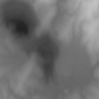
\includegraphics[width=0.4\textwidth]{figures/samp_orig.png}
	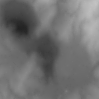
\includegraphics[width=0.4\textwidth]{figures/samp_comp.png}
	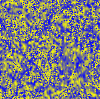
\includegraphics[width=0.4\textwidth]{figures/samp_diff.png}
	\caption{From the~top to the~bottom - the~original terrain, the~same terrain compressed with the~maximum deviation of 5m, the~difference between these~two. The~brighter the~color, the~greater the~value. In the~difference image, the~yellow color means 4.5m, whereas the~blue color means -4.5m.}
	\label{fig:result_samples}
\end{figure}

\newcommand{\incexampl}[1]{\includegraphics[width=0.225\textwidth]{#1}}

\begin{figure}
	\incexampl{figures/dim_64_amp_16_lon_4_horizontal_orig.png}
	\incexampl{figures/dim_64_amp_16_lon_16_horizontal_orig.png}\\\\
	\incexampl{figures/dim_64_amp_16_lon_4_horizontal_out.png}
	\incexampl{figures/dim_64_amp_16_lon_16_horizontal_out.png}\\\\
	\incexampl{figures/dim_64_amp_16_lon_4_horizontal_diff.png}
	\incexampl{figures/dim_64_amp_16_lon_16_horizontal_diff.png}
	\caption{Two synthetic test images of size 64x64, each one containing spiky terrain with the~heights ranging from -16 to 16. On the~left, the~longitude of spikes is 4, on the~right, it is 16. From the~top to the~bottom - the~original, compressed with the~maximum deviation of 5, the~difference between these~two. The~brighter the~color, the~greater the~value. In the~difference image, the~yellow color means 4.5, whereas the~blue color means -4.5.}
	\label{fig:result_wave_samples}
\end{figure}